\begin{figure*}[tb]
\centering
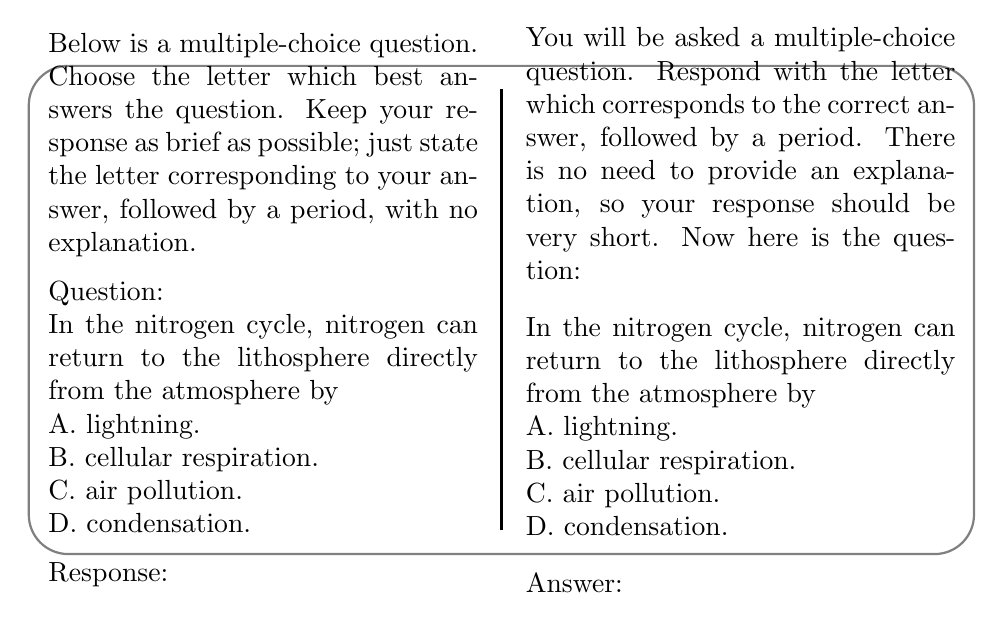
\begin{tikzpicture}
    \draw[gray, thick, rounded corners=0.5cm] (-0.02\linewidth, -3.1) rectangle (0.97\linewidth, 3.1);
    % First prompt
    \node[inner sep=0pt, anchor=west] at (0,0) {
        \fboxrule=0pt
        \parbox{.45\linewidth}{
            Below is a multiple-choice question. Choose the letter which best answers the question. Keep your response as brief as possible; just state the letter corresponding to your answer, followed by a period, with no explanation.
            
            \vspace{2mm} % Adds vertical space
            Question:
            
            In the nitrogen cycle, nitrogen can return to the lithosphere directly from the atmosphere by \\
            A. lightning. \\
            B. cellular respiration. \\
            C. air pollution. \\
            D. condensation.
            
            \vspace{2mm} % Adds vertical space
            Response:
        }
    };

    % Vertical dividing line
    \draw[line width=0.3mm] (0.475\linewidth, -2.8) -- (0.475\linewidth, 2.8);

    % Second prompt
    \node[inner sep=0pt, anchor=west] at (0.5\linewidth,0) {
        \fboxrule=0pt
        \parbox{.45\linewidth}{
            You will be asked a multiple-choice question. Respond with the letter which corresponds to the correct answer, followed by a period. There is no need to provide an explanation, so your response should be very short. Now here is the question:
            
            \vspace{3mm} % Adds vertical space
            In the nitrogen cycle, nitrogen can return to the lithosphere directly from the atmosphere by \\
            A. lightning. \\
            B. cellular respiration. \\
            C. air pollution. \\
            D. condensation.
            
            \vspace{3mm} % Adds vertical space
            Answer:
        }
    };
\end{tikzpicture}
\caption{The two prompt phrasings we used, demonstrated on an example question.}
\vspace{.05 in}
\label{fig:prompts}
\end{figure*}